\section{Platformy streamingowe}
Ogromny potencjał drzemiący w analizie danych w czasie rzeczywistym został dostrzeżony przez wiele firm.
Dlatego pierwsze rozwiązania powstawały wewnątrz departamentów \textit{IT},
dopiero potem będąc upublicznionym.
Dzięki temu na rynku dostępnych jest wiele rozwiązań oferujących analizę strumieniową.
Poprzez rozwiązania komercyjne od gigantów jak Microsoft, Google, Amazon,
po typu \textit{open-source},
takie jak Apache Storm, Apache Spark czy Apache Flink.

Wśród rozwiązań \textit{open-source} kilka cieszy się dość ugruntowaną pozycją na rynku,
przekładającą się na wiele udanych wdrożeń.
Są to:
\begin{itemize}
	\item Esper,
	\item Apache Spark,
	\item Apache Storm.
\end{itemize}

Powyższe plaformy zostały wybrane do dalszej analizy z uwagi na swoją dojrzałość.
Cieszą się dużą popularnością oraz mają aktywną społeczność,
co jest bardzo ważne podczas planowania i wyboru architektury rozwiązania.

\subsection{Esper}
Esper firmy EsperTech Inc. jest silnikiem umożliwiającym złożoną analizę zdarzeń
(\textit{Complex Event Processing, CEP}).
możliwym do osadzenia w dowolnej aplikacji Java lub .Net.
Esper dzięki swojemu bardzo ekspresywnemu językowi umożliwia na swobodne manipulowanie strumieniami danych.

Język Esper to specjalnie przygotowany język domenowy (\textit{domain specific language, DSL}) do obsługi zdarzeń.
Język ma formę zapytań (kwerend) i został oparty na standardzie \textit{SQL}.

\begin{lstlisting}[captionpos=b, caption=Przykładowe zapytanie w języku Esper]
  select * from StockTickEvent(symbol='IBM').win:length(100)
\end{lstlisting}

Niewątpliwie jedną z głównych zalet Espera jest jego prostota instalacji.
Wystarczy dołączyć bibliotekę,
która jest w formie pojedynczego pliku \textit{jar}
do aplikacji i rozwiązanie jest gotowe do użytku.
Kolejną zaletą jest język dający szerokie pole do działania.
Dzięki oparciu go o klasyczny \textit{SQL} język ten jest zrozumiały dla osób dopiero rozpoczynających naukę,
jak i dla osób bez podstaw informatycznych.
Dostępne funkcje to:
filtrowanie wyników
\begin{lstlisting}
  select * from
    StockTickEvent
  where symbol='IBM'
\end{lstlisting}
funkcje agregujace
\begin{lstlisting}
  select symbol, avg(value) as value from
    StockTickEvent
  group by symbol
\end{lstlisting}
funkcje grupujące (\textit{window functions})
\begin{lstlisting}
  select * from
    StockTickEvent.win:length(100)
\end{lstlisting}
łączenie strumieni
\begin{lstlisting}
  select * from
    TickEvent.std:unique(symbol) as t,
    NewsEvent.std:unique(symbol) as n
  where t.symbol = n.symbol
\end{lstlisting}
tworzenie nowych strumieni
\begin{lstlisting}
  insert into IbmStockTickEvent
  select * from
    StockTickEvent
  where symbol='IBM'
\end{lstlisting}

Niestety to co okazało się zaletą Espera czyli prostota instalacji
jest także jego wadą.
Esper nie ma żadnych wbudowanych mechanizmów ułatwiających skalowanie,
tj. jest tak samo skalowalny jak aplikacja w której został osadzony.

Esper nie daje żadnych gwarancji przetworzenia wiadomości.
Przetwarzane wiadomości znajdują się wyłącznie w pamięci komputera (\textit{in-memory}),
nie są w żaden sposób nigdzie zapisywane,
tak więc w razie awarii węzła tracone są bezpowrotnie.

\subsection{Apache Spark}
Apache Spark jest narzędziem mającym swoje początki na uniwersytecie Berkley.
Jest to ogólnego przeznaczenia framework do zadań obliczeniowych,
charakteryzujący się dobrymi właściwościa skalowania.
Wykorzystywany jest z powodzeniem w operacjach związanych z:
\begin{itemize}
  \item uczeniem maszynowym,
  \item klasteryzacją dużej ilości danych,
  \item analizą strumieniową.
\end{itemize}

% napisany w scali

Jednym z ciekawych elementów tego frameworka
jest możliwość korzystania z jego API w innych językach niż tylko z rodziny jvm (\textit{Java Virtual Machine}).
Oprócz scali czy javy dostepne są:
\begin{itemize}
  \item python
  \item R
\end{itemize}

% moduly
% jak dziala
% zalety

\subsection{Apache Storm}
Apache Storm jest frameworkiem umożliwiającym strumieniowe przetwarzanie danych w czasie rzeczywistym.
Charakteryzuje się przy tym:
\begin{itemize}
  \item skalowalnością,
  \item odpornością na awarię,
  \item niezawodnością.
\end{itemize}
Stworzony został przez inżynierów z firmy
Backtype (Marz, 2014),
a po jej przejęciu, rozwijany przez inżynierów Twittera.
Obecnie projekt został otwarty publicznie dla społeczności \textit{open-source}
i jest nadzorowany przez fundację Apache.

\subsubsection*{Elementy składowe Storm}
\label{subs:StormElemets}
W przypadku Storma reprezentacja zadania nazywana jest topologią (\textit{topology}).
Jest to acykliczny graf skierowany (rys. \ref{fig:StormTopology}).
Elementami grafu są strumienie danych,
elementy tworzące strumień (\textit{spouts})
i elementy operacyjne (\textit{bolts}).
Topologie Storm koncepcyjnie zbliżone są do zadań z przetwarzania wsadowego.
Różnią się tym,
że gdy zadania wsadowe mają jasno określone momenty startu i końca,
to topologię działają nieprzerwanie, do czasu gdy zostaną jawnie zatrzymane.
\begin{figure}[htbp]
  \centering
  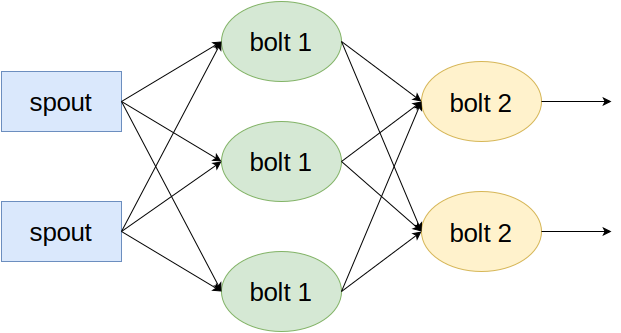
\includegraphics[width=0.9\textwidth]{img/storm}
  \caption{Topologia Storm}
  \label{fig:StormTopology}
\end{figure}

\subsubsection*{Strumienie}
Podstawową strukturą danych w systemach Storm jest krotka (\textit{tuple}).
Krotka jest zbiorem par klucz-wartość przepływających pomiędzy elementami topologi.
Krotka w połączeniu z innymi krotkami tworzy strumień danych.
\subsubsection*{Spouts}
\textit{Spouts} reprezentują punkty wejścia krotek do topologi Storm.
Strumienie mają właśnie swój początek w elementach typu \textit{spouts}.
Przykładowo mogą to być:
\begin{itemize}
  \item dane z sensorów, czujników,
  \item informacje z serwisów społecznościowych,
  \item logi aplikacyjne.
\end{itemize}
\subsubsection*{Bolts}
\textit{Bolts} są elementami w topologiach,
w których wykonywana jest właściwa praca na danych.
Mogą przyjmować na wejście dowolną liczbę strumieni,
przeprocesować je
i jeśli zajdzie taka potrzeba stworzyć nowe strumienie.
\textit{Bolts} mogą podłączać się do strumieni generowanych przez \textit{spouts},
jak i do innych \textit{bolts}.
Dzięki temu można tworzyć skomplikowane struktury przepływów strumieni danych.
Typowymi zastosowaniami \textit{bolts} są:
\begin{itemize}
  \item filtrowanie,
  \item preprocesowanie danych (oczyszczanie, standaryzowanie formatów),
  \item operacje biznesowe,
  \item zapisy w bazach danych.
\end{itemize}

\subsubsection*{Mechanizmy procesowania rozproszonego}
Storm od początku projektowany był z myślą o procesowaniu rozproszonym,
pozwalającym na łatwe skalowanie horyzontalne.
Zadania dzielone są na wiele niezależnych od siebie pod-zadań,
które mogą być uruchamiane równolegle na wielu maszynach na raz.

Elementy ułatwiające realizację wymagań można podzielić na cztery główne grupy.
\begin{enumerate}
  \item Węzły (\textit{nodes}) są pojedynczymi maszynami podłączonymi do klastra Storm,
  na których wykonywane są topologie.
  \item Procesy (\textit{workers}) są fizyczne procesy uruchamiane na węzłach.
  Na jednym węźle może być uruchomionych więcej niż jeden proces.
  \item Wątki (\textit{executors}) są to standardowe wątki uruchomiana wewnątrz procesów.
  \item Zadania (\textit{tasks}) są instancjami obiektów typu \textit{spouts} i \textit{bolts}.
  Operacje są wywoływane przez wątki.
\end{enumerate}
Zależności elementów pomiędzy sobą przedstawiono na rysunku \ref{fig:StormParallel}.
\begin{figure}[htbp]
  \centering
  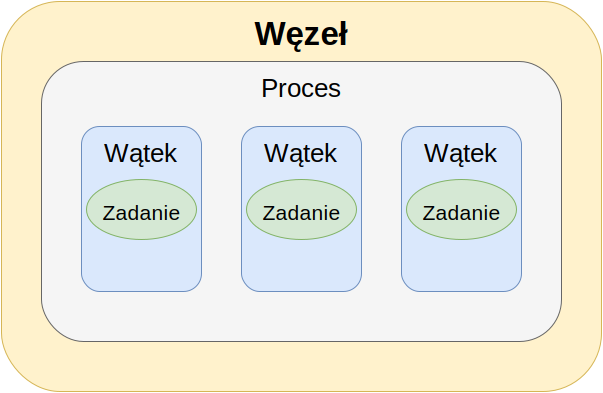
\includegraphics[width=0.8\textwidth]{img/stormElements}
  \caption{Elementy tworzące topologię Storm}
  \label{fig:StormParallel}
\end{figure}

\subsubsection*{Zarządzanie klastrem}
Klaster Storma wykorzystuje klasyczne podejście \textit{master}/\textit{slave}
jednak w trochę innym znaczeniu.
W architekturze typu \textit{master}/\textit{slave} najczęściej jest jeden węzeł nadrzędny (\textit{master}),
który jest wcześniej zapisany w konfiguracji
bądź jest wybierany dynamicznie po starcie.
W przypadku Storma zostało zastosowane drugie podejście.
Klaster Storma (rys. \ref{fig:StormCluster}) składa się z jednego węzła \textit{master} nazywanego \textit{nimbus}
i jednego bądź więcej węzłów pomocniczych nazywanych zarządcami (\textit{supervisors})
Dodatkowo do koordynacji komunikacji pomiędzy nimbusem,
a zarządcami wykorzystywany jest Apache ZooKeeper.
\begin{figure}[htbp]
  \centering
  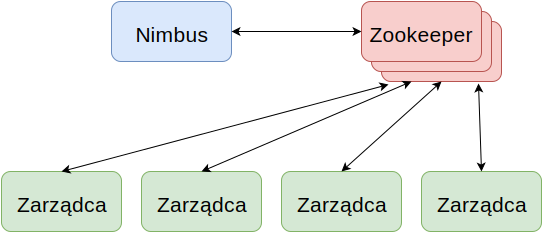
\includegraphics[width=0.8\textwidth]{img/stormCluster}
  \caption{Elementry klastra Storm}
  \label{fig:StormCluster}
\end{figure}

Węzeł \textit{nimbus} jest odpowiedzialny za zarządzanie,
koordynowanie i monitorowania wszystkich topologi pracujących w klastrze.
Dodatkowo zajmuje się także przydziałem zadań dla krotek
oraz pilmowaniem by wszystkie zadania zostały wykonane.
W przypadku awiarii \textit{nimbus} uruchamia ponownie zadanie w innym miejscu klastra.
Węzeł zarządzający odpowiedzialny jest za przydział zadań otrzymanych z \textit{nimbusa}.
Tworzy nowy procesy (\textit{workers}) w ramach węzła,
przydziele do nich zadania.

